\documentclass[11pt]{article}

\usepackage[utf8]{inputenc}
\usepackage[T1]{fontenc}

\usepackage[a4paper,total={210mm,297mm},left=25mm,right=25mm,top=25mm,
bottom=25mm]{geometry}

\usepackage[portuguese]{babel}

\usepackage{lastpage}
\usepackage{graphicx}
\usepackage{caption}
\usepackage{subcaption}
\graphicspath{{figs/}}

\usepackage{fancyhdr}
\pagestyle{fancy}
\fancyhead[L]{POO}
\fancyhead[C]{Relatório de Projecto}
\fancyhead[R]{Junho 2021}
\renewcommand{\footrulewidth}{0.4pt}
\cfoot{\thepage\ / \pageref{LastPage}}

\date{\vspace{-5ex}}

\title{Programação Orientada aos Objetos

Relatório de Projeto - Grupo 21}

\author{
	A93324 Daniel Torres Azevedo  \
	\and
	A70573 Mário Rui Sendas Rocha
	\and
	A42865 Mário Rui Freitas Coelho \
}

\begin{document}

\maketitle

\begin{figure}[h!]
	\centering
	\begin{subfigure}[h!]{0.3\linewidth}
		\centering
		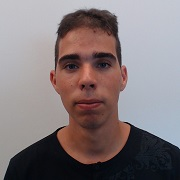
\includegraphics[width=\linewidth]{Daniel.jpeg}
		A93324 Daniel
	\end{subfigure}%
	\begin{subfigure}[h!]{0.3\linewidth}
		\centering
		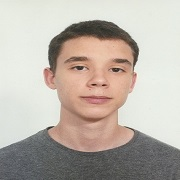
\includegraphics[width=\linewidth]{Mario.jpeg}
		A70573 Mário
	\end{subfigure}%
	\begin{subfigure}[h!]{0.3\linewidth}
		\centering
		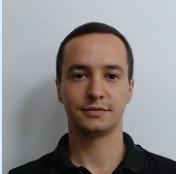
\includegraphics[width=\linewidth]{MC.jpeg}
		A42865 Mário Coelho
	\end{subfigure}
\end{figure}


\section{Introdução}
Este trabalho realizado no âmbito da unidade curricular de Programação Orientada aos Objetos tem o objetivo de desenvolver uma aplicação para criar um sistema de gestão e simulação de equipas. Embora se pretenda que o sistema seja versátil e adaptável a qualquer desporto, no presente relatório apresenta-se o caso particular do futebol a titulo ilustrativo.

Esta aplicação permite simular a existência de um conjunto de jogadores, agrupados em equipas. É possível também simular a realização de jogos de futebol.

\section{Arquitetura da Aplicação}
Esta aplicação segue o modelo MVC (Model View Control), onde uma classe esta encarregada da comunicação com o usuário, a View, outra esta encarregada do processamento da informação, o Model, e uma terceira, o Control, que faz a "ponte" entre estas duas, isto é, recebe a informação do usuário, envia-a para o model e envia os resultados do model para o View para serem mostrados.

Este padrão de arquitetura foi implementado com recurso à utilização de \textit{Interfaces} de modo a permitir ocultar a implementação de cada componente. Assim, no futuro será possível por exemplo:

\begin{enumerate}

\item alterar a view, por exemplo substituindo a interface textual por uma interface gráfica, bastando para isso implementar uma nova classe (com a referida interface gráfica) que implemente a interface \textit{IView} e, por consequência, os respetivos métodos;

\item alterar o model, por exemplo substituindo a atual lógica de negócio centrada no futebol, por uma outra lógica de negócio relacionada com um outro desporto. Para tal, bastará desenvolver uma nova classe que implemente a interface \textit{IModel};

\item alterar o control, em função de alguma (ou ambas) das alterações referidas acima, de modo a conseguir responder às novas funcionalidades que venham a ser implementadas. Neste caso, a interface que o novo control teria de implementar seria, naturalmente, a interface \textit{IControl}.

\end{enumerate}

Todas as três interfaces foram implementadas seguindo a seguinte estrutura de código:

\begin{itemize}

\item \underline{métodos abstratos}: cuja implementação ficará a cargo das classes que implementem a interface;

\item \underline{constantes}: que passariam a estar disponíveis em qualquer classe que implemente a respetiva interface;

\item \underline{métodos default}: cuja implementação seria fornecida pela própria interface;

\item \underline{métodos static}: semelhantes aos anteriores, mas disponíveis a partir da própria interface;

\end{itemize}

\subsection{Model}
A classe Model contém a lógica de negócio. Assim, é dentro desta classe que reside o coração da aplicação e da funcionalidade que desta se espera.

É esta classe que chama depois todas as classes detalhadas na secção seguinte e que traduzem os conceitos que a aplicação pretendia modelar.

Em particular, as classes \textit{Jogador}, e as suas várias especializações (tipos de jogador), bem como a classe \textit{Equipa}


\subsection{Control}
Como dito anteriormente, o control é a classe "intermediária" da arquitetura MVC, este contem um objeto da classe View e outro da class Model, e faz a ligação entre os mesmos.

Esta classe é também responsável por gerir as tarefas de input e output, tendo para tal um conjunto de métodos que permitem receber do utilizador informação e devolver ao utilizador as respostas adequadas.

\subsection{View}
Por último, na classe view são incluídos todo um conjunto de conteúdos gráficos sob a forma de menus. De facto, sendo a aplicação baseada numa interface textual, os elementos gráficos a mostrar ao utilizador final são essencialmente linhas de texto.

No entanto, de modo a dar algum aspeto dinâmico à aplicação, procurou-se que os menus fossem variando e se fossem adaptando a cada momento de interação com o utilizador.

\section{Classes}

Nesta secção detalha-se um pouco as principais classes que constituem a aplicação desenvolvida.

Para todas as classes, seguindo as boas práticas aprendidas ao longo do semestre, procurou-se o mais possível seguir a seguinte estruturação do código:

\begin{itemize}
\item \underline{variáveis de instância}: disponíveis a qualquer instância da respetiva classe;

\item \underline{variáveis de classe}: que passariam a estar disponíveis diretamente a partir da classe;

\item \underline{construtores}: pelo menos os seguintes três foram considerados havendo, no entanto, margem para a consideração de outros mais específicos caso necessário.

\subitem \textit{vazio}

\subitem \textit{paramétrico}

\subitem \textit{cópia}

\item \underline{getters e setters}: responsáveis por ler ou escrever as/nas variáveis de instância. Deste modo garantia-se desde logo o encapsulamento de cada classe;
 
\item \underline{métodos override}: a implementar sempre que se pretenda substituir algum método cuja implementação exista por defeito. Nesta categoria inserem-se, por exemplo, os métodos \textit{toString}, \textit{equals} e \textit{clone};

\item \underline{métodos abstratos}: a implementar obrigatoriamente caso se esteja a implementar alguma interface;

\item \underline{métodos específicos}: cuja implementação só faz sentido no contexto de instâncias da respetiva classe;

\item \underline{métodos static}: semelhantes aos anteriores, mas disponíveis a partir da própria classe e não de instâncias suas;

\end{itemize}

\subsection{Jogador(es)}
Uma vez que os vários tipos de jogadores apenas diferem em algumas variáveis de instância, optou-se por recorrer a uma superclasse \textit{Jogador} onde tudo o que fosse comum aos demais jogadores ficaria agrupado.

No entanto, pelo facto de que cada tipo de jogador tem uma forma distinta de quantificar a sua habilidade, a superclasse \textit{Jogador} foi tornada abstrata. O seu principal método abstrato era precisamente o método \textit{habilidade}, que seria calculado de forma distinta para cada tipo de jogador.

Na Tabela \ref{tab:habilidade} apresentam-se os pesos relativos que foram considerados para calcular a habilidade de cada tipo de jogador. Destacam-se as três características especificas dos jogadores do tipo Guarda-redes, Médio e Lateral. Uma vez que estas classes traduziam funcionalidades especificas destes tipos de jogador, procurou-se que o peso relativo destas fosse substancialmente superior às demais.

Nos restantes jogadores, procurou-se dar mais importância às características mais relevantes para cada posição.

\begin{table}[!h]
	\centering
	\caption{Pesos adotados na quantificação da habilidade de cada tipo de jogador.}
	\label{tab:habilidade}
	\begin{tabular}{|l|l|l|l|l|l|}
		\hline
		Jogador      & Guarda-redes & Defesa & Médio & Avançado & Lateral \\ \hline
		Velocidade   & 0.1          & 0.2    & 0.05  & 0.05     & 0.1     \\ \hline
		Resistência  & 0.1          & 0.2    & 0.05  & 0.05     & 0.1     \\ \hline
		Destreza     & 0.2          & 0.05   & 0.05  & 0.05     & 0.15    \\ \hline
		Impulsão     & 0.2          & 0.2    & 0.1   & 0.2      & 0.1     \\ \hline
		Cabeça       & 0            & 0.2    & 0.1   & 0.2      & 0.1     \\ \hline
		Remate       & 0            & 0.05   & 0.2   & 0.4      & 0.1     \\ \hline
		Passe        & 0.1          & 0.1    & 0.05  & 0.05     & 0.1     \\ \hline
		Elasticidade & 0.3          & -      & -     & -        & -       \\ \hline
		Cruzamento   & -            & -      & -     & -        & 0.25    \\ \hline
		Recuperação  & -            & -      & 0.4   & -        & -       \\ \hline
	\end{tabular}
\end{table}

Em termos de implementação, para além das variáveis de instância visíveis na Tabela \ref{tab:habilidade}, foi ainda considerada uma variável para guardar o estado possível de cada jogador ao longo do jogo (\textit{SUPLENTE, TITULAR, SAINDO, ENTRANDO}) e uma outra, do tipo lista, com o historial de equipas por onde o jogador passou.

Por último, foi também considerada uma variável de classe que guardaria um contador dos jogadores existentes no sistema. Deste modo garante-se que não existem dois jogadores iguais no sistema

\subsection{Equipa e Jogo}

As restantes duas principais classes da aplicação eram a Equipa e o Jogo. Contrariamente à classe Jogador, nestas não foi considerado o uso de um contador global uma vez que se pressupõe que não existem duas equipas com o mesmo nome, no caso da classe Equipa, nem dois jogos exatamente iguais, no caso da classe Jogo.

Para além das necessárias variáveis de instância, e respetivos métodos getters e setters, estas classes implementaram algumas das funcionalidades especificas de cada uma.

No caso da Equipa, foi implementado um método \textit{habilidade} semelhante ao existente para os Jogadores. Na verdade, é um método que se limita a chamar o método homónimo em cada jogador da equipa e soma o total da habilidade de todos os jogadores.


\subsection{Exceções}

Tendo em conta as funcionalidades implementadas na aplicação, foram consideradas essencialmente dois tipos de exceções. Tanto para o caso dos jogadores como para as equipas, essas exceções correspondem aos cenários em que ou a instância (de jogador/equipa) que está a ser solicitada pelo utilizador não existe no sistema ou já existe uma cópia da mesma pelo que não é possível criar uma nova instância igual.

\section{Conclusão}

O desenvolvimento do presente trabalho revelou-se um desafio interessante para o grupo. Foi possível experienciar alguns dos principais problemas que surgirão, no futuro profissional, num projeto semelhante. A aplicação das técnicas e metodologias aprendidas ao longo do semestre revelaram que, efetivamente, ter hábitos de boas práticas de programação e dividir o problema maior em pequenos problemas mais pequenos permitem abordar com sucesso o desenvolvimento de aplicações.

Chegados a esta fase das conclusões do trabalho, e tendo a clara noção de que muito poderia ser melhorado, detalham-se de seguida alguns dos aspetos a melhorar numa próxima revisão da aplicação:

\begin{itemize}

\item desenvolver uma sistema de base de dados que, à medida que a aplicação fosse utilizada, permitisse ir guardando os dados de utilização da mesma. Assim, seria possível convergir para uma aplicação mais semelhante à que serviu de inspiração ao presente trabalho;

\item conforme o trabalho foi idealizado, existem muitos parâmetros que tiveram de ser arbitrados. Isso poderia ser revisto numa próxima versão através do fornecimento de um ficheiro de logs mais completo que o atualmente existente;

\item apesar de se terem previsto e tratado algumas das possíveis exceções, existem muitas outras que não foram abordadas que seguramente beneficiariam a aplicação caso o fossem no futuro;

\end{itemize}

\newpage

\section*{Anexo - Diagrama de classes}

\begin{figure}[!h]
	\centering
	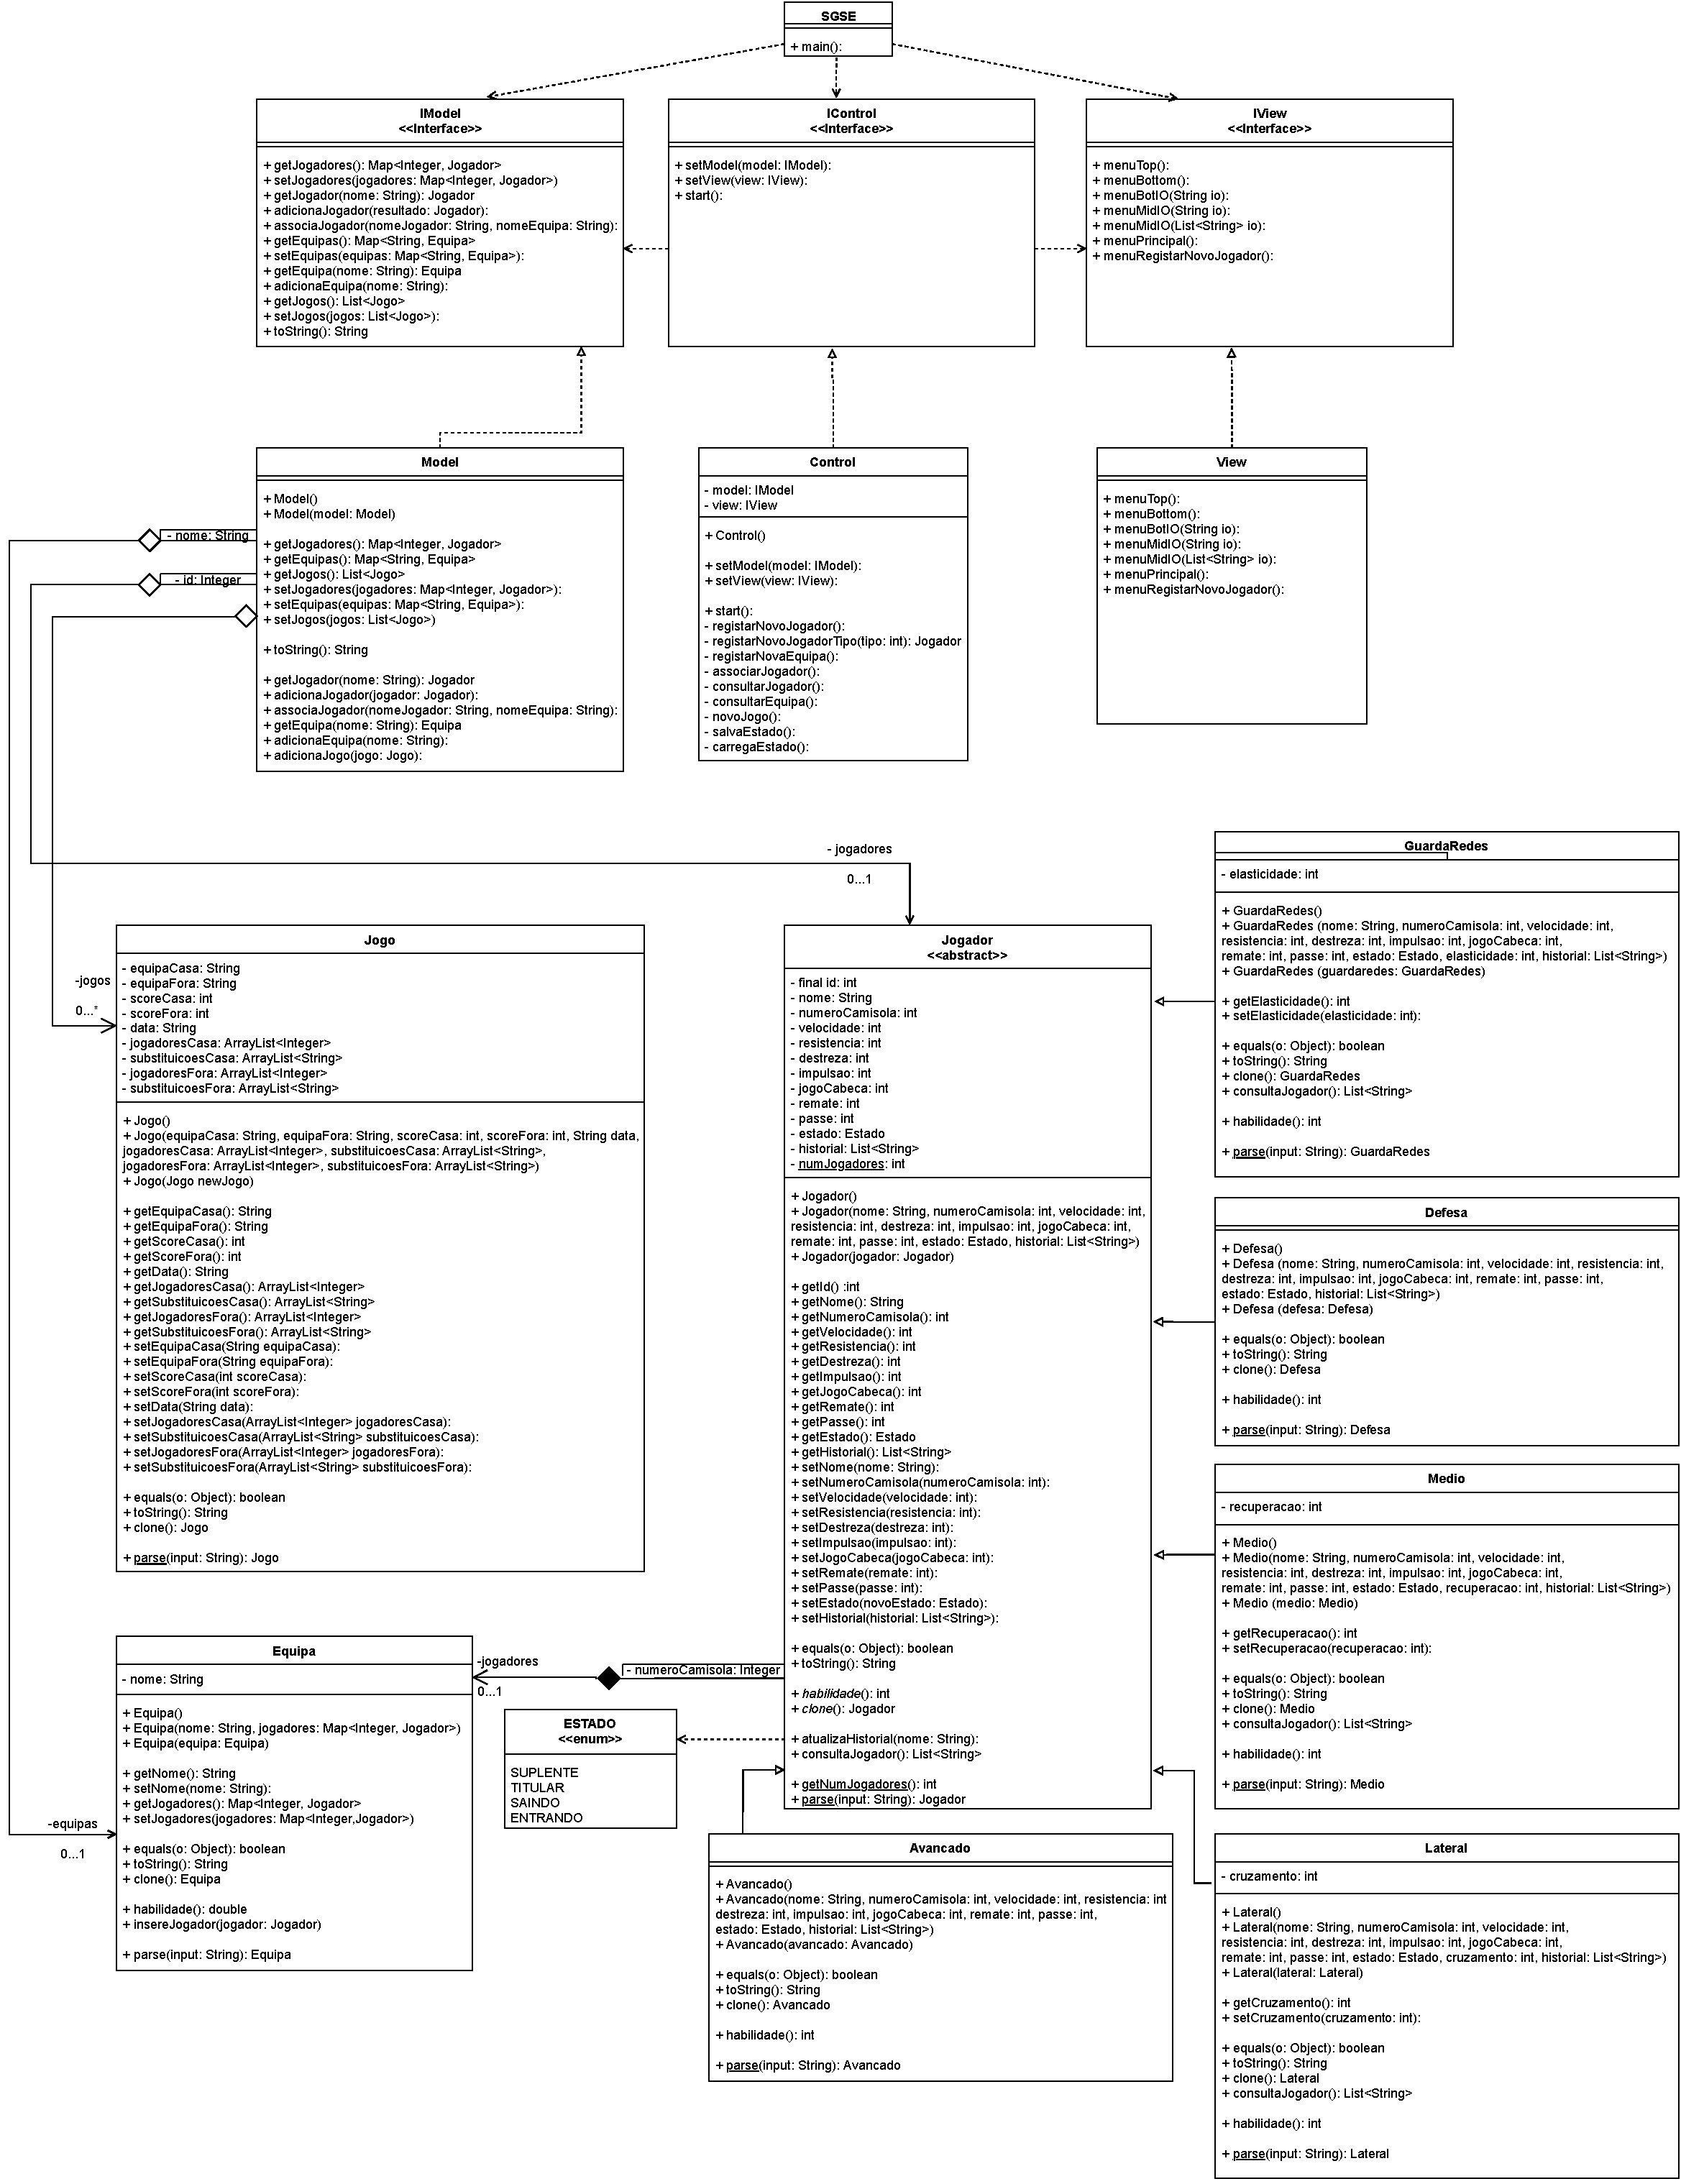
\includegraphics[height=0.8\textheight]{Diagrama.pdf}
	\caption{Diagrama de classes do projeto.}
	\label{fig:diagramaClasses}
\end{figure}

\end{document}
